% !TEX TS-program = pdflatex
% !TEX encoding = UTF-8 Unicode

% This is a simple template for a LaTeX document using the "article" class.
% See "book", "report", "letter" for other types of document.

\documentclass[12pt]{report} % use larger type; default would be 10pt

\usepackage[utf8]{inputenc} % set input encoding (not needed with XeLaTeX)

%%% Examples of Article customizations
% These packages are optional, depending whether you want the features they provide.
% See the LaTeX Companion or other references for full information.

%%% PAGE DIMENSIONS
\usepackage{geometry} % to change the page dimensions
\geometry{a4paper} % or letterpaper (US) or a5paper or....
% \geometry{margin=2in} % for example, change the margins to 2 inches all round
% \geometry{landscape} % set up the page for landscape
%   read geometry.pdf for detailed page layout information

\usepackage{graphicx} % support the \includegraphics command and options

% \usepackage[parfill]{parskip} % Activate to begin paragraphs with an empty line rather than an indent

%%% PACKAGES
\usepackage{booktabs} % for much better looking tables
\usepackage{array} % for better arrays (eg matrices) in maths
\usepackage{paralist} % very flexible & customisable lists (eg. enumerate/itemize, etc.)
\usepackage{verbatim} % adds environment for commenting out blocks of text & for better verbatim
\usepackage{subfig} % make it possible to include more than one captioned figure/table in a single float
\usepackage[final]{pdfpages}
% These packages are all incorporated in the memoir class to one degree or another...

%%% HEADERS & FOOTERS
\usepackage{fancyhdr} % This should be set AFTER setting up the page geometry
\pagestyle{fancy} % options: empty , plain , fancy
\renewcommand{\headrulewidth}{0pt} % customise the layout...
\lhead{}\chead{}\rhead{}
\lfoot{}\cfoot{\thepage}\rfoot{}

%%% SECTION TITLE APPEARANCE
\usepackage{sectsty}
\allsectionsfont{\sffamily\mdseries\upshape} % (See the fntguide.pdf for font help)
% (This matches ConTeXt defaults)

%%% RULE

\newcommand{\HRule}{\rule{\linewidth}{0.5mm}}

%%% BIBLIOGRAPHY

\usepackage{apacite}                           %bibliography in apa-style

%%% ToC (table of contents) APPEARANCE
\usepackage[nottoc,notlof,notlot]{tocbibind} % Put the bibliography in the ToC
\usepackage[titles,subfigure]{tocloft} % Alter the style of the Table of Contents
\renewcommand{\cftsecfont}{\rmfamily\mdseries\upshape}
\renewcommand{\cftsecpagefont}{\rmfamily\mdseries\upshape} % No bold!

\setcounter{secnumdepth}{-2}

%%% TABLES

\renewcommand{\arraystretch}{1.2}

%%% END Article customizations

%%% The "real" document content comes below...

\begin{document}

\begin{titlepage}

\begin{center}


% Upper part of the page

\includegraphics[width=1\textwidth]{./logo}\\[1cm]    

\textsc{\Large Bachelor Thesis}\\[0.5cm]
\textsc{\Large {[}201000166{]}}\\[0.5cm]


% Title
\HRule \\[0.4cm]
{ \huge \bfseries Teaching quantum mechanics using qCraft}\\[0.4cm]

\HRule \\[1.5cm]

% Author and supervisor
\begin{minipage}{0.4\textwidth}
\begin{flushleft} \large
\emph{Author:}\\
Micha \textsc{van den Enk} \\
{[}s1004654{]} \\
\end{flushleft}
\end{minipage}
\begin{minipage}{0.4\textwidth}
\begin{flushright} \large
\emph{Supervisors:} \\
Dr. H. H. \textsc{Leemkuil} \\
Second \textsc{supervisor} \\
\end{flushright}
\end{minipage}

\vfill

% Bottom of the page
{\large \today}

\end{center}

\end{titlepage}

\setcounter{tocdepth}{1}
\tableofcontents
\newpage

\section{Preface}

%%% ANALYSIS

\section{The Generic Model}

\begin{figure}[h]
\centering
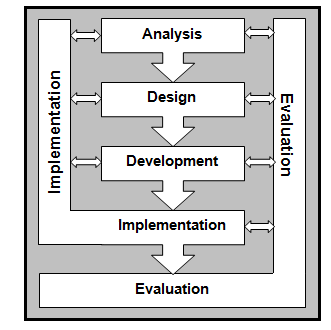
\includegraphics[width=0.7\textwidth]{genericmodel}
\caption{\footnotesize The generic model by \protect\citeA{genericmodel}\label{fig:genericmodel}}
\end{figure}

\chapter{Analyses}

The first step of the Generic Model by \citeA{genericmodel} (see figure~\ref{fig:genericmodel} on page~\pageref{fig:genericmodel}) is Analysis. \citeA{smithragan} give an elaborated description of how to perform these analyses for instructional design. They distinguish three different kinds of analysis: analyzing the learner context, analyzing the learner and analyzing the learning task. The analysis of the learning context can provide the instructional needs and a description of the different factors influencing the instruction. The purpose of the learner analysis is the characterization of the end user of the instruction, which is in this case the middle school students. In the task analysis the test specifications are written, with which the content of the instruction can be established.These three analyses are executed in the following three chapters.

% Context Analysis

\section{Context Analysis}

A learning task always takes place in a certain learning context. In this case this is the middle school. It entails not only the place, but also the temporal and social environment \cite{smithragan}. The analysis of the learning context can provide the instructional needs and a description of the different factors influencing the instruction. With the instructional needs, the designer can establish the main learning goals for the instruction. The description of the learning environment can provide the learning opportunities and constraints which have to be taken into account for the instruction.

%needs assessment

\subsection{Needs Assessment}

The first goal of the need assessment is to investigate whether there exists a need for the instruction.  Without a need, it would be a waste of resources to develop the instruction \cite{smithragan}. Next to this, it is conducted to better specify the need for the instruction. In the context of instruction, the assessment often results in a learning goal, which is the main goal of the instruction. This main goal is needed to continue the rest of the analyses, because all other analyses are conducted in respect to this goal. The goal can also be used to construct the summative evaluation, because when this goal is achieved, the instruction has proved to be successful.

\paragraph{The condition}

\citeA{smithragan} identify three different models for the needs assessment, namely the problem model, the innovation model and the discrepancy model (see figure~\ref{fig:needsassessment}). The problem model is used when there exists a problem in the current system which has to be solved. As can be seen in figure~\ref{fig:needsassessment}, this model is to be used as a prerequisite for the other two models for assessment. With this model, it is determined whether there really is a problem, whether the cause of the problem is related to emloyees' performance or learners' achievement, whether the solution to the problem is learning and whether instruction for these learning goals is currently offered. After the problem model, the needs assessment splits into the two other models. The innovation model is used when there is a new learning goal that the learners should achieve, and the discrepancy model is used when the already available instruction is not adequate to achieve the learning goal. The designer should choose one of these models for his needs assessment.

\begin{figure}[h]
\centering
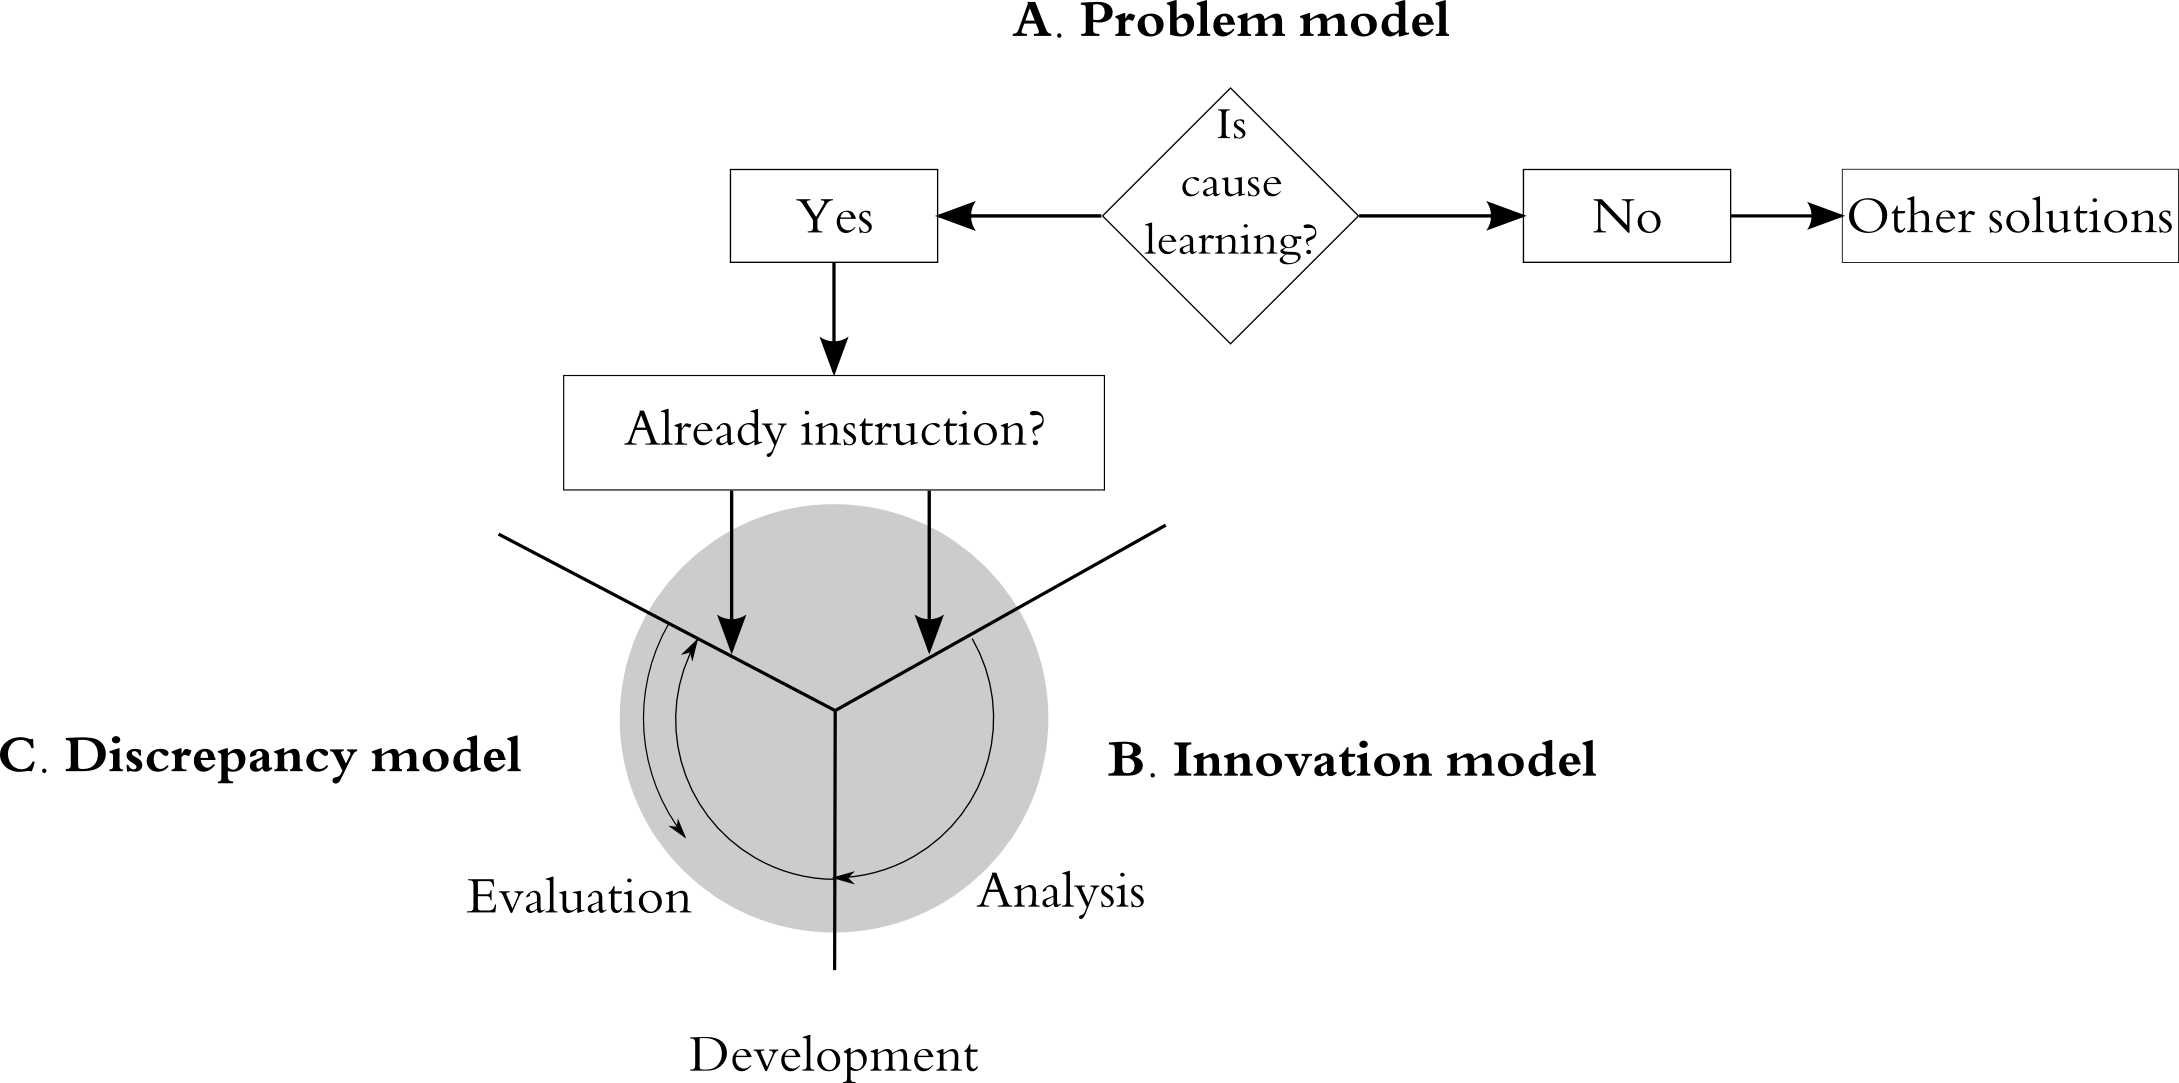
\includegraphics[width=\textwidth]{needsassessment}
\caption{\footnotesize The three sides of needs assessment \protect\cite{smithragan}\label{fig:needsassessment}}
\end{figure}

In the case of the instruction which will be constructed for this assignment, at first the problem model will be used to investigate the problem, and which of the two follow-up models should be used for the needs assessment.

\paragraph{The problem}



\paragraph{Cause of the problem}

\paragraph{Is the solution learning}

\paragraph{Instruction currently offered}

\paragraph{Nature of the innovation}

\paragraph{Learning goals}

\paragraph{Priority and suitability}

%learning environment

\subsection{Learning Environment}

The learning environment description is the other major component of the learning context analysis \cite{smithragan}. The description contains information of all the external factors influencing the instruction. These are the mediators of the instruction, the already existing curricula which takes place in the environment, the available equipment available on the location of the instruction, the characteristics of the facilities at the location of the instruction, the characteristics of the organization in which the instruction will take place, and the philosophies and ta boos of the larger community in which this organization exists.

\paragraph{Teachers}

\paragraph{Existing curricula}

\paragraph{Equipment}

\paragraph{Facilities}

\paragraph{Organization}

\paragraph{Larger system}

% Learner analysis

\section{Learner Analysis}

The second analysis is that of the learners \cite{smithragan}. The purpose of this analysis is the characterization of the end user of the instruction, which is in this case the middle school students. For this analysis it is important to determine the similarities and differences between the learners. \citeA{smithragan} provide a list of factors which play a role in designing the instruction. They catagorize these factors with a ${2 \times 2}$ matrix (see table~\ref{tab:learneranalysis}), creating the catagories stable similarities, changing similarities, stable differences, and changing differences.

\begin{table}[h]
\begin{center}
\begin{tabular}{| l | l | l |}
\hline
 & \textbf{Similarities} & \textbf{Differences} \\ \hline
\textbf{Stable} & Stable similarities & Stable differences \\ \hline
\textbf{Changing} & Changing similarities & Changing differences \\ \hline
\end{tabular}
\end{center}
\caption{\footnotesize The four catagories of Learner Characteristics \protect \cite{smithragan} \label{tab:learneranalysis}}
\end{table}

%stable similarities

\subsection{Stable Similarities}

\paragraph{Sensory capacities}

\paragraph{Information processing}

\paragraph{Types and conditions of learning}

%changing similarities

\subsection{Changing Similarities}

\paragraph{Intellectual development processes}

\paragraph{Language development processes}

\paragraph{Psychosocial development processes}

\paragraph{Moral development processes}

\paragraph{Other development processes}

%stable differences

\subsection{Stable Differences}

\paragraph{Aptitudes}

\paragraph{Cognitive styles}

\paragraph{Psychosocial traits}

\paragraph{Gender, ethnicity, \& racial group}

%changing differences

\subsection{Changing Differences}

\paragraph{Intellectual development state}

\paragraph{Other development state}

\paragraph{General prior learning}

\paragraph{Specific prior learning}

% Task analysis

\section{Task Analysis}

The final step is analyzing the learning task \cite{smithragan}. In this analysis the goals from the needs assessment during the analysis of the learning context have to be translated to test specifications, with which the content of the instruction can be established. In order to achieve these test specifications, first the type of learning has to be established. Having this established, the information-processing analysis can be conducted. Every type of learning has its own kind of information-processing analysis. \citeA{dance} provides a clear conceptual understanding of quantum teleportation, and will therefore be used to conduct this information-processing analysis. The next step is the prerequisite analysis. The outcome of this has to correspond to the outcome of the learner analysis. Finally, the learning objectives can be written, which form the test specifications. Every learning objective has to contain a description of the terminal behaviour or actions that will demonstrate learning, a description of the conditions of demonstration of that action and a description of the standard or criterion \cite{smithragan}. Every learning objective will fall into a category of Bloom his taxonomy of learning objectives \cite{bloom}, and will use appropriate action verbs. Most learning objectives within will be knowledge objectives, because there is a lot of new knowledge which has to be provided and it forms the basis for all other objectives. There will be no or very few synthesis and evaluation objectives, because these objectives would take too much time within the instruction to achieve to be feasible to use.

\subsection{Learning goal}

\subsection{Types of learning}

\subsection{Information-processing analysis}

\subsection{Prerequisite analysis}

\subsection{Learning objectives}

\subsection{Test specifications}

% Theoretic Framework

\chapter{Theoretic Framework}

%%% DESIGN

\chapter{Design}

%%% DEVELOPMENT

\chapter{Development}

%%% FORMATIVE EVALUATION

\chapter{Formative Evaluation}

\bibliographystyle{apacite}
\bibliography{references}

\end{document}
